\subsection{Pishahang Results}
The \ref{fig:pishcirroscase1180-cpu} \ref{fig:pishcirroscase1180-mem} and \ref{fig:pishahang-top-3-lifecycle} shows the CPU utilization, memory utilization and CPU utilization through out the life cycle of Pishahang dockers during the experiment respectively. Let us consider the important dockers in each case and list their functionalities to realize why they have consumed maximum CPU.


\subsubsection{CPU}

The \ref{fig:cirroscase1180-cpu} shows CPU utilization. The first 6 Pishahang dockers are:

\begin{itemize}
	\item \textbf{son-sp-infrabstract:} This docker plays the role of an abstraction layer between the MANO framework and the underlying virtualised infrastructure. It exposes the interfaces to manage services and the VNF instances of all of these 180 instances by reserving resources for their service deployment. It also receives monitoring information about the infrastructure status. Hence, it occupies much of the CPU.
	\item \textbf{sevicelifecyclemanagement:} This is responsible for orchestrating the entire lifecycle of every service that is being deployed with Pishahang service platform. The lifecycle operations of NS include
	
	\begin{itemize}
		\item \textit{NS operations:} 
		1) On-board Network Service
		2) Instantiate Network Service
		3) Scale Network Service
		4) Update Network Service by supporting Network Service configuration changes
		Create, delete, query, and update of VNFFGs associated to a Network Service.
		5) Terminate Network Services
		
	\end{itemize}

	\item \textbf{son-broker:} The Pishahang service platform consists of micro services that use a message broker to communicate, building a flexible orchestration system.
	
The load on all of the other microservices in Pishahang service platform is distributed and the difference between their mean usage is negligible. Hence, the order of all other microservices can be insignificant.

	
	\item \textbf{specificmanageregistry:} The role of this docker is to manage lifecycle of FSM (function-specific manager) and SSM(service-specific manager). Lifecycle operations of FSM and SSM include instantiation, registeration, updation and termination. ex: to obtain onboarding SSM request from SLM.
	\item \textbf{cloudservicelifecyclemanagement:}This docker is responsible for lifecycle management of cloud network services on kubernates.
	\item \textbf{functionallifecyclemanagement:}  This docker manages the lifecycle events of each VNF in these 180 network instances. 

\begin{itemize}
		
	\item \textit{VNF operations:} 1) Instantiate VNF (create a VNF using the VNF on-boarding artefacts)
	2) Scale VNF (increase or reduce the capacity of the VNF).
	3) Update and/or Upgrade VNF (support VNF software and/or configuration changes of various complexity).
	4) Terminate VNF (release VNF-associated NFVI resources and return it to NFVI resource pool)
\end{itemize}
	\end{itemize}

\begin{figure}[h]
	\centering
	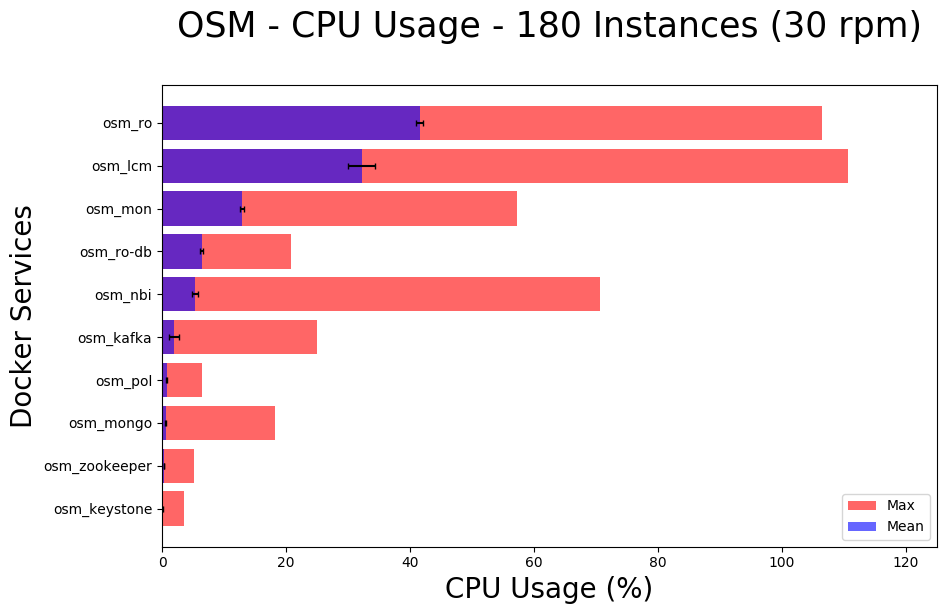
\includegraphics[width=0.7\linewidth]{../figures/scalability_graphs/Horizontal-Docker-Graphs/pishahang/cirros_case1_180-CPU}
	\caption{Pishahang CPU}
	\label{fig:pishcirroscase1180-cpu}
\end{figure}
\pagebreak
\subsubsection{Memory Utilization}
The first 5 Pishahang dockers in memory utilization graph \ref{fig:pishcirroscase1180-mem} are:

\begin{itemize}
	\item \textbf{son-keyclock:} This docker service provides access management and identity management of these micro services.
	\item \textbf{son-monitor-influxdb:} This monitoring plugin records metrics on the internal runtime and service performance and writes it to database.
	\item \textbf{son-sp-infrabstract:}  This docker plays the role of an abstraction layer between the MANO framework and the underlying virtualised infrastructure. It exposes the interfaces to manage services and the VNF instances of all of these 180 instances by reserving resources for their service deployment. It also receives monitoring information about the infrastructure status. Hence, it occupies much of the memory.
	
	\item \textbf{WIM adaptor:} The role of this microservice is to provide connectivity over the physical network. The WIM adaptor acts as a north-bound interface to the higher layers,T eg., NFVO to provide connectivity services between NFVI-POPs or to physical network functions. This also invokes the underlying NFVI network southbound interfaces, whether they are network controllers or NFs, to construct the service within the domain.
	
	\item \textbf{son-gtksrv:} This is Pishahang's gatekeeper service management micro-service.
	
\end{itemize}
 The most important inference from \ref{fig:cirroscase1180-mem} and \ref{fig:pishcirroscase1180-mem} is that, the memory utilisation by Pishahang is much lighter than OSM for the top docker services.



\begin{figure}[h]
	\centering
	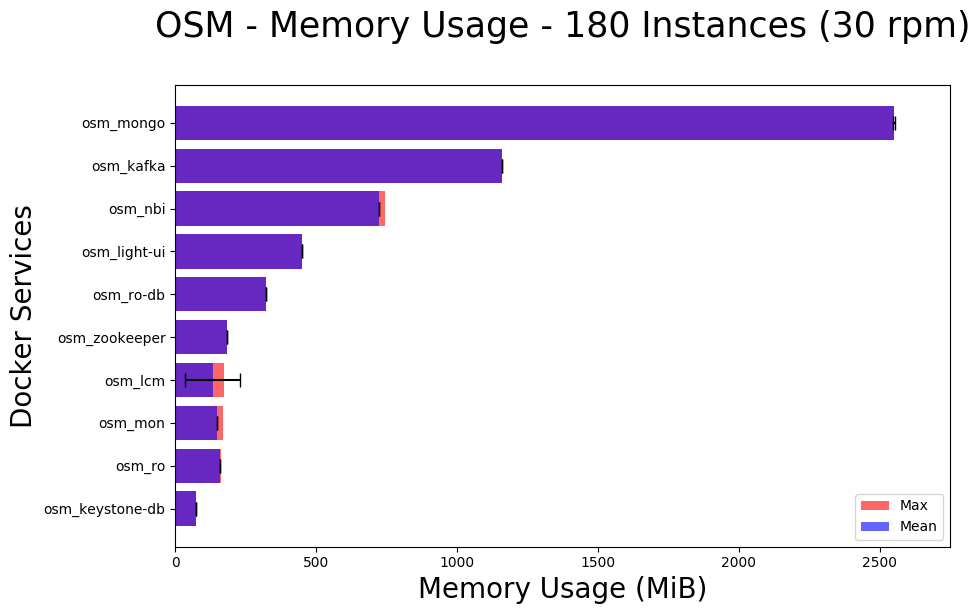
\includegraphics[width=0.7\linewidth]{../figures/scalability_graphs/Horizontal-Docker-Graphs/pishahang/cirros_case1_180-MEM}
	\caption{Pishahang MEM}
	\label{fig:pishcirroscase1180-mem}
\end{figure}
\pagebreak

\subsubsection{Lifecycle}

We now have the life cycle graphs of the entire experiment. The \ref{fig:pishahang-top-3-lifecycle} shows the distribution of the CPU usage among the top 3 dockers throughout the experiment. The experiment lasted for about 10 minutes.

Initially, the metrics of docker containers are recorded for one minute, which can be visualized in \ref{fig:pishahang-top-3-lifecycle} with almost no significant change in the CPU occupancy. The Pishahang infrastructure was reserved for all the 180 instances and with termination requests over the time, the CPU usage was reduced like before. This is observed by the graph of son-sp-infrabstract docker. The graph also depicts the CPU occupancy of other top docker services throughout the experiment.


\begin{figure}[h]
	\centering
	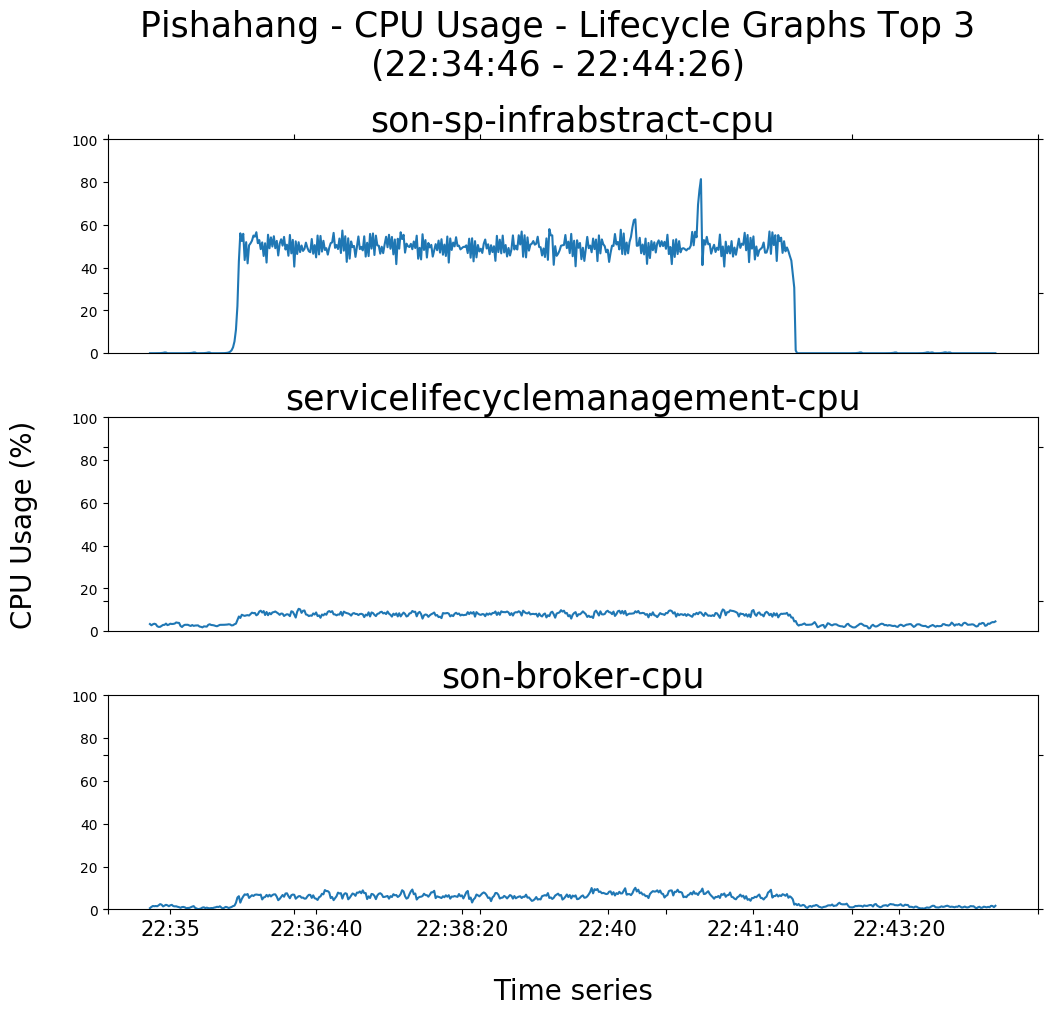
\includegraphics[width=0.7\linewidth]{figures/scalability_graphs/Lifecycle-Graphs-Top-3/Pishahang-TOP-3-Lifecycle}
	\caption{Pish LS}
	\label{fig:pishahang-top-3-lifecycle}
\end{figure}
